% Qualitative-analysis paragraph

A provisional single reviewer visual audit of 56 POPE hallucinations identified three recurring mechanisms. Localized visual confusion occurs when a compact false cue resembles the queried object. One Qwen 7B example asks whether a car is present in an airport scene. The model answers yes with $p_{\mathrm{yes}}=0.936$, while the hidden evidence map concentrates on a ground-service vehicle. Blurring the top hidden patch changes the answer to no and reduces $p_{\mathrm{yes}}$ to $0.048$; blurring a matched random patch leaves the answer at yes with $p_{\mathrm{yes}}=0.931$. Diffuse scene priors occur when broad context, such as a market or dining scene, supports an object without a compact cue. Semantic or annotation ambiguity occurs when the queried category is arguably visible but absent from the benchmark label, such as a clock on a desk. These labels are qualitative and require independent review before they should be treated as a formal taxonomy result.

\begin{figure*}[t]
\centering
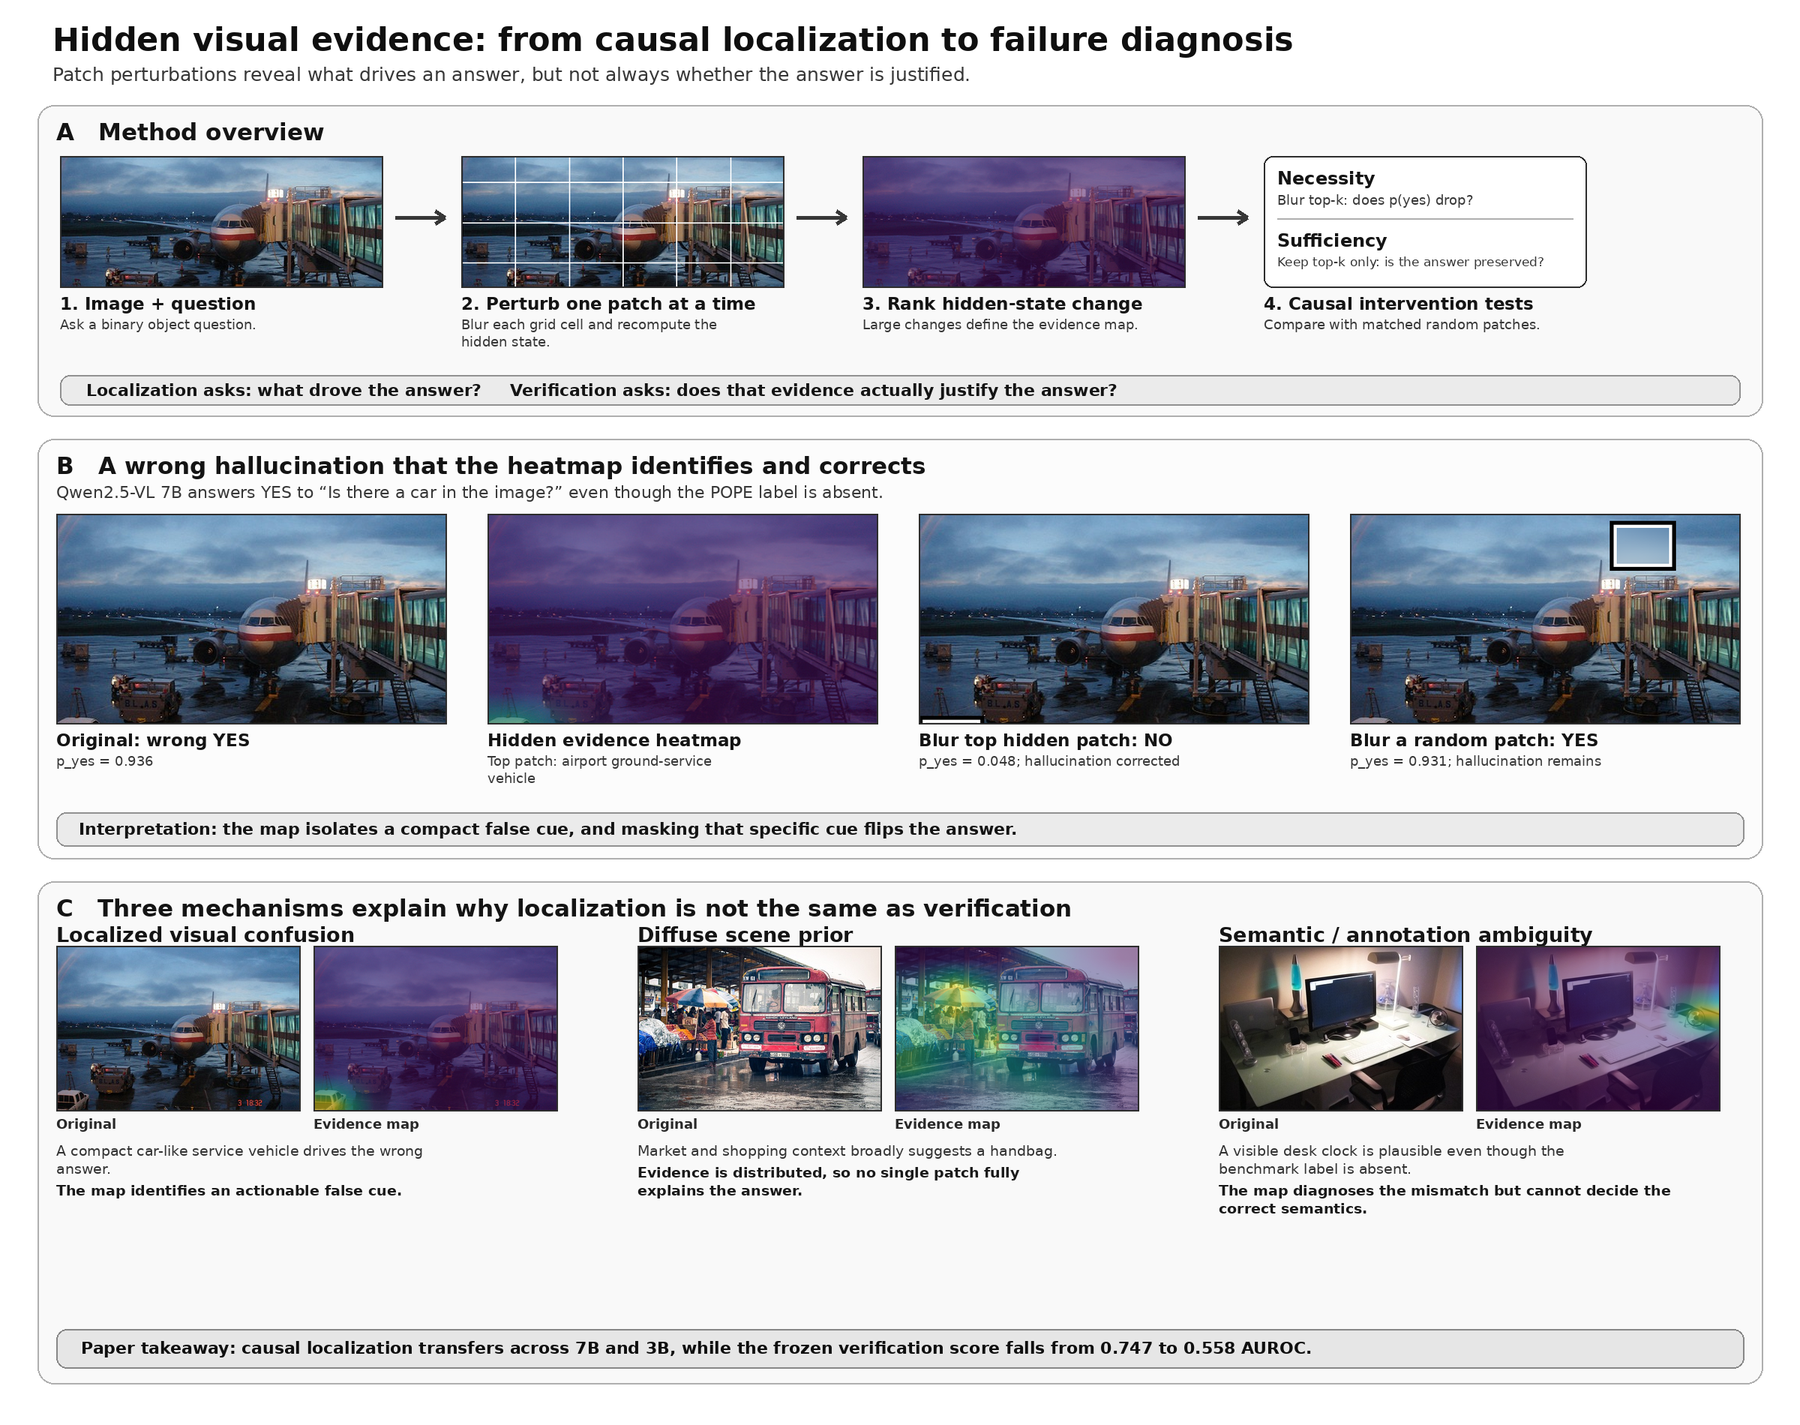
\includegraphics[width=\textwidth]{figures/headline_method_taxonomy_figure_paper.png}
\caption{Method and failure taxonomy. Patchwise blur interventions rank regions by hidden-state change, followed by matched necessity and sufficiency tests. In the airport example, Qwen 7B hallucinates a car with $p_{\mathrm{yes}}=0.936$ because a compact ground-service vehicle acts as a false cue. Blurring the top hidden patch corrects the answer and lowers $p_{\mathrm{yes}}$ to $0.048$, while a random blur leaves the hallucination nearly unchanged. The remaining examples illustrate diffuse scene priors and semantic or annotation ambiguity, explaining why causal localization does not by itself provide semantic verification.}
\label{fig:taxonomy}
\end{figure*}
